Firstly, it is easy find that naphthalene belongs to the point group $\mathscr{D}_{\rm 2h}$, whose character table is shown in \Tableref{tab:chatab_5}.		
		\begin{center}
		\setlength{\abovecaptionskip}{0em}
		\captionof{table}{The character table for the $\mathscr{D}_{\rm 2h}$ point group.}\label{tab:chatab_5}
		\begin{tabular}{ccccccccc}\hline
	$\mathscr{D}_{\rm 2h}$ & $E$ & $C_{2z}$ &	$C_{2y}$	& $C_{2x}$	&	$i$	&	$\sigma_{xy}$	&	$\sigma_{xz}$ &	$\sigma_{yz}$\\ \hline
			$A_g$		&	1	&	1	&	1	&	1	&	1	&	1	&	1	&	1	\\
			$B_{1g}$	&	1	&	1	&	-1	&	-1	&	1	&	1	&	-1	&	-1	\\
			$B_{2g}$ 	&	1	&	-1	&	1	&	-1	&	1	&	-1	&	1	&	-1	\\
			$B_{3g}$ 	&	1	&	-1	&	-1	&	1	&	1	&	-1	&	-1	&	1	\\ 
			$A_u$		&	1	&	1	&	1	&	1	&	-1	&	-1	&	-1	&	-1	\\
			$B_{1u}$	&	1	&	1	&	-1	&	-1	&	-1	&	-1	&	1	&	1	\\
			$B_{2u}$ 	&	1	&	-1	&	1	&	-1	&	-1	&	1	&	-1	&	1	\\
			$B_{3u}$ 	&	1	&	-1	&	-1	&	1	&	-1	&	1	&	1	&	-1	\\ \hline
		\end{tabular}
		\end{center}
		
		Secondly, we mark all carbon atoms as follows.
		\begin{center}
		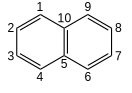
\includegraphics[scale=1.0]{./structures/exercise_1/naphthalene/0.png}
		\setlength{\abovecaptionskip}{-0.3em}
		\captionof{figure}{The order of carbon atoms in naphthalene.}
		\setlength{\belowcaptionskip}{-0.8em}
		\end{center}	
		
		For $\pi$-electron atomic orbitals' representation $\Gamma^{\rm AO}$, its following characters is listed below.		
		\begin{center}
		\setlength{\abovecaptionskip}{-0.3em}
		\captionof{table}{The character of the $\pi$-electron atomic orbitals' representation $\Gamma^{\rm AO}$.}
		\begin{tabular}{ccccccccc}\hline
	$\mathscr{D}_{\rm 2h}$	& $E$ & $C_{2z}$ &	$C_{2y}$	& $C_{2x}$	&	$i$	$\sigma_{xy}$	&	$\sigma_{xz}$	&	$\sigma_{xz}$ &	$\sigma_{yz}$  \\ \hline
	$\chi^{\AO}(C_i)$	&	10	&	0	&	-2	&	0	&	0	&	-10	&	0	&	2	\\ \hline
		\end{tabular}\vspace*{-0.5em}
		\end{center}
		Relevant reduction coefficients are
		\begin{align*}
			a_g = 0,	\quad	b_{1g} = 0,	\quad	b_{2g} = 2,	\quad	b_{3g} = 3,	\quad a_u = 2,	\quad b_{1u} = 3,	\quad	b_{2u} = 0,	\quad	b_{3u} = 0.
		\end{align*}
		Thus, we arrive at
		\begin{equation*}
			\Gamma^{\AO} = 2\Gamma^{B_{2g}} \oplus 3\Gamma^{B_{3g}} \oplus 2\Gamma^{A_u} \oplus 3\Gamma^{B_{1u}}.
		\end{equation*}
		We conclude that there are three basis functions in the irreducible representation $\Gamma^{B_{3g}}$ and $\Gamma^{B_{1u}}$, respectively. Thus, to describe the effect of $O_R$, three suitable $2 \orbp_z$ atomic orbitals $\phi_i$ is enough.
		
		\begin{center}
		\setlength{\abovecaptionskip}{0em}
		\captionof{table}{Transformation of $\phi_i$ under $O_R$ for the naphthalene.}
		\begin{tabular}{ccccccccc}\hline
	$\mathscr{D}_{\rm 5}$ & $E$ & $C_{2z}$ & $C_{2y}$ & $C_{2x}$	&	$i$	&	$\sigma_{xy}$ &	$\sigma_{xz}$	&	$\sigma_{yz}$\\ \hline
			$\phi_1$	&	$\phi_1$	&	$\phi_6$	&	$-\phi_9$	&	$-\phi_4$	&	$-\phi_6$	&	$-\phi_1$	&	$\phi_4$	&	$\phi_9$		\\
			$\phi_2$	&	$\phi_2$	&	$\phi_7$	&	$-\phi_8$	&	$-\phi_3$	&	$-\phi_7$	&	$-\phi_2$	&	$\phi_3$	&	$\phi_8$		\\ 
			$\phi_5$	&	$\phi_5$	&	$\phi_{10}$	&	$-\phi_5$	&	$-\phi_{10}$	&	$-\phi_{10}$	&	$-\phi_5$	&	$\phi_{10}$	&	$\phi_5$		\\\hline
		\end{tabular}
		\end{center}
		
		For the irreducible representation $\Gamma^{B_{2g}}$, the only two basis functions are
		\begin{align*}
			P^{B_{2g}}\phi_1 &= \sum_{R} \chi^{B_{2g}}(R) O_R \phi_1 = 2(\phi_1 + \phi_4 - \phi_6 - \phi_9 ), \\
			P^{B_{2g}}\phi_2 &= \sum_{R} \chi^{B_{2g}}(R) O_R \phi_2 = 2(\phi_2 + \phi_3 - \phi_7 - \phi_8 ).	
		\end{align*}
		They can be normalized to
		\begin{align*}
			\phi^\prime_1 &= \frac{1}{2}(\phi_1 + \phi_4 - \phi_6 - \phi_9), \\
			\phi^\prime_2 &= \frac{1}{2}(\phi_2 + \phi_3 - \phi_7 - \phi_8).
		\end{align*}
		Besides, it is easy to find that they are mutually orthogonal.
		
		Then, the effective Hamiltonian for $\pi$ electrons is
		\begin{equation*}
			H^\prime_{B_{2g}} = \begin{pmatrix}
				\alpha	&	\beta	\\
				\beta	&	\alpha+\beta
				\end{pmatrix}.				
		\end{equation*}
		Its eigen equation is		
		\begin{equation}
			\det(\Hp_{B_{2g}}-\varepsilon^\pi \Sp_{B_{2g}}) = \beta^2 ( x^2 + x - 1 ) = 0.
		\end{equation}
		There are two roots,
		\begin{equation}
			x_1 = \frac{-1+\sqrt{5}}{2}, \quad x_2 = \frac{-1-\sqrt{5}}{2},
		\end{equation}
		which equal to
		\begin{align}
			\varepsilon^\pi_1 &= \alpha - \frac{\sqrt{5}-1}{2}\beta, \\
			\varepsilon^\pi_2 &= \alpha + \frac{\sqrt{5}+1}{2}\beta.
		\end{align}
		
		For $\Hp_{B_{2g}}-\varepsilon^\pi_1 \Sp_{B_{2g}}$, its reduced row echelon form is
		\begin{equation*}
			\begin{pmatrix}
				1	& \frac{1+\sqrt{5}}{2}	\\	0	&	0
			\end{pmatrix},
		\end{equation*}
		which means
		\begin{equation*}
			\Phi_1 = \frac{\sqrt{5}+1}{2}\phi^\prime_1 - \phi^\prime_2.
		\end{equation*}
		The sum of squares of coefficients is
		\begin{equation*}
			\sum_{i} c^2_i = \frac{ 5+\sqrt{5} }{2},
		\end{equation*}
		Thus, we know
		\begin{align}
			\Phi^\pi_1 &= \sqrt{ \frac{2}{5+\sqrt{5}} } \Phi_1 = \sqrt{ \frac{2}{5+\sqrt{5}} } \left[ \frac{\sqrt{5}+1}{2}\phi^\prime_1 - \phi^\prime_2 \right] = \sqrt{\frac{\sqrt{5}+1}{2\sqrt{5}}} \phi^\prime_1 - \sqrt{\frac{\sqrt{5}-1}{2\sqrt{5}}} \phi^\prime_2	\notag \\
			&= \frac{1}{2}\sqrt{\frac{\sqrt{5}+1}{2\sqrt{5}}} (\phi_1 + \phi_4 - \phi_6 - \phi_9) - \frac 12 \sqrt{\frac{\sqrt{5}-1}{2\sqrt{5}}} (\phi_2 + \phi_3 - \phi_7 - \phi_8)\notag \\
			&\approx 0.4253 \phi_1 - 0.2629 \phi_2 - 0.2629 \phi_3 + 0.4253 \phi_4 - 0.4253\phi_6 + 0.2629\phi_7 + 0.2629\phi_8 - 0.4253 \phi_9.
		\end{align}
		
		Similarly, the reduced row echelon form of $\Hp_{B_{2g}}-\varepsilon^\pi_2 \Sp_{B_{2g}}$ is
		\begin{equation*}
			\begin{pmatrix}
				1	& \frac{1-\sqrt{5}}{2}	\\	0	&	0
			\end{pmatrix},
		\end{equation*}		
		which means
		\begin{equation*}
			\Phi_2 = \frac{\sqrt{5}-1}{2}\phi^\prime_1 + \phi^\prime_2.
		\end{equation*}
		And then,
		\begin{align}
			\Phi^\pi_2 &= \sqrt{ \frac{2}{5-\sqrt{5}} } \Phi_2 = \sqrt{\frac{\sqrt{5}-1}{2\sqrt{5}}} \phi^\prime_1 + \sqrt{\frac{\sqrt{5}+1}{2\sqrt{5}}} \phi^\prime_2	\notag \\
			&= \frac{1}{2}\sqrt{\frac{\sqrt{5}+1}{2\sqrt{5}}}(\phi_1 + \phi_4 - \phi_6 - \phi_9) + \frac{1}{2}\sqrt{\frac{\sqrt{5}-1}{2\sqrt{5}}} (\phi_2 + \phi_3 - \phi_7 - \phi_8) \notag \\
			&\approx 0.2629 \phi_1 + 0.4253 \phi_2 + 0.4253 \phi_3 + 0.2629 \phi_4 - 0.2629\phi_6 - 0.4253 \phi_7 - 0.4253 \phi_8 - 0.2629 \phi_9.
		\end{align}

		In conclusion, for the irreducible representation $\Gamma^{B_{2g}}$, relevant results are listed below.
		
		\begin{center}
		\setlength{\abovecaptionskip}{0em}
		\captionof{table}{The H{\"u}ckel MOs in the irreducible representation $\Gamma^{B_{2g}}$ of naphthalene.}
		\begin{tabular}{ccccccc}\hline
		order & eigenvalue & \multicolumn{5}{c}{eigenfunction} \\ \hline
		\multirow{4}*{1}	&	\multirow{4}*{$\alpha-0.618\beta$}	&	$c_1$	&	$c_2$	&	$c_3$	&	$c_4$	&	$c_5$	\\	\cline{3-7}
			&	&	0.4253 &	- 0.2629	&	- 0.2629	&	0.4253	&	0.0000	\\	\cline{3-7}
			&	&	$c_6$	&	$c_7$	&	$c_8$	&	$c_9$	&	$c_{10}$	\\	\cline{3-7}
			&	&	- 0.4253	&	0.2629	&	0.2629	&	- 0.4253	&	0.0000	\\	\hline
		\multirow{4}*{2}	&	\multirow{4}*{$\alpha+1.618\beta$}	&	$c_1$	&	$c_2$	&	$c_3$	&	$c_4$	&	$c_5$	\\	\cline{3-7}
			&	&	0.2629 &	0.4253	&	0.4253	&	0.2629	&	0.0000	\\	\cline{3-7}
			&	&	$c_6$	&	$c_7$	&	$c_8$	&	$c_9$	&	$c_{10}$	\\	\cline{3-7}
			&	&	- 0.2629	&	-0.4253	&	- 0.4253	&	-0.2629	&	0.0000	\\	\hline
		\end{tabular}
		\end{center}
		
		For the irreducible representation $\Gamma^{B_{3g}}$, the only three basis functions are
		\begin{align*}
			P^{B_{3g}}\phi_1 &= \sum_{R} \chi^{B_{3g}}(R) O_R \phi_1 = 2(\phi_1 - \phi_4 - \phi_6 + \phi_9 ), \\
			P^{B_{3g}}\phi_2 &= \sum_{R} \chi^{B_{3g}}(R) O_R \phi_2 = 2(\phi_2 - \phi_3 - \phi_7 + \phi_8 ),  \\
			P^{B_{3g}}\phi_5 &= \sum_{R} \chi^{B_{3g}}(R) O_R \phi_5 = 4(\phi_5- \phi_{10} ).
		\end{align*}
		They can be normalized to
		\begin{align*}
			\phi^\prime_3 &= \frac{1}{2}(\phi_1 - \phi_4 - \phi_6 + \phi_9), \\
			\phi^\prime_4 &= \frac{1}{2}(\phi_2 - \phi_3 - \phi_7 + \phi_8), \\
			\phi^\prime_5 &= \frac{1}{\sqrt{2}}(\phi_5 - \phi_{10}).
		\end{align*}
		Besides, it is easy to find that they are mutually orthogonal.
		
		Then, the effective Hamiltonian for $\pi$ electrons is
		\begin{equation*}
			H^\prime_{B_{3g}} = \begin{pmatrix}
				\alpha	&	\beta	&	-\sqrt{2}\beta	\\
				\beta	&	\alpha-\beta	&	0		\\
				-\sqrt{2}\beta	&	0	&\alpha-\beta
				\end{pmatrix}.				
		\end{equation*}
		Its eigen equation is		
		\begin{equation*}
			\det(\Hp_{B_{2g}}-\varepsilon^\pi \Sp_{B_{2g}}) = \beta^3 (x-1)( x^2 - x - 3 ) = 0.
		\end{equation*}
		There are three roots,
		\begin{equation*}
			x_3 = 1, \quad x_4 = \frac{1+\sqrt{13}}{2}, \quad x_2 = \frac{1-\sqrt{13}}{2},
		\end{equation*}
		which equal to
		\begin{align}
			\varepsilon^\pi_3 &= \alpha - \beta, \\
			\varepsilon^\pi_4 &= \alpha - \frac{1+\sqrt{13}}{2}\beta \approx \alpha - 2.303 \beta, \\
			\varepsilon^\pi_5 &= \alpha + \frac{\sqrt{13}-1}{2}\beta \approx \alpha + 1.303 \beta.
		\end{align}
		
		For $\Hp_{B_{3g}}-\varepsilon^\pi_3 \Sp_{B_{3g}}$, its reduced row echelon form is
		\begin{equation*}
			\begin{pmatrix}
				1	& 0	&	0	\\	0	&	1	&	-\sqrt{2}	\\	0	&	0	&	0
			\end{pmatrix},
		\end{equation*}
		which means
		\begin{equation*}
			\Phi_3 = \sqrt{2}\phi^\prime_4 + \phi^\prime_5.
		\end{equation*}
		The sum of squares of coefficients is
		\begin{equation*}
			\sum_{i} c^2_{3,i} = 3,
		\end{equation*}
		Thus, we know
		\begin{align}
			\Phi^\pi_3 &= \sqrt{\frac{2}{3}} \phi^\prime_4 + \sqrt{\frac{1}{3}} \phi^\prime_5	\notag \\
			&= \sqrt{\frac{1}{6}} (\phi_2 - \phi_3 +\phi_5 - \phi_7 + \phi_8 -\phi_{10})  \notag \\
			&\approx 0.4082 \phi_2 - 0.4082 \phi_3 + 0.4082 \phi_5 -  0.4082\phi_7 + 0.4082 \phi_8 - 0.4082 \phi_{10}.
		\end{align}
		
		Similarly, the reduced row echelon form of $\Hp_{B_{3g}}-\varepsilon^\pi_4 \Sp_{B_{3g}}$ is
		\begin{equation*}
			\begin{pmatrix}
				1	& 0	&	-\frac{\sqrt{13}-1}{2\sqrt{2}}	\\	0	&	1	&	\frac{1}{\sqrt{2}}	\\	0	&	0	&	0
			\end{pmatrix},
		\end{equation*}		
		which means
		\begin{align*}
			\Phi_4 &= \frac{\sqrt{13}-1}{2\sqrt{2}}\phi^\prime_3 - \frac{1}{\sqrt{2}} \phi^\prime_4 + \phi^\prime_5.
		\end{align*}
		The sum of squares of coefficients is
		\begin{equation*}
			\sum_{i} c^2_{4,i} = \frac{13-\sqrt{13}}{4}.
		\end{equation*}
		And then,
		\begin{align}
			\Phi^\pi_4 &= \frac{2}{\sqrt{13-\sqrt{13}}} \Phi_4 = \sqrt{\frac{\sqrt{13}-1}{2\sqrt{13}}} \phi^\prime_3 - \sqrt{\frac{\sqrt{13}+1}{6\sqrt{13}}} \phi^\prime_4	+ \sqrt{\frac{\sqrt{13}+1}{3\sqrt{13}}} \phi^\prime_5\notag \\
			&= \frac{1}{2}\sqrt{\frac{\sqrt{13}-1}{2\sqrt{13}}}(\phi_1 - \phi_4 - \phi_6 + \phi_9) - \frac{1}{2}\sqrt{\frac{\sqrt{13}+1}{6\sqrt{13}}} (\phi_2 - \phi_3 - \phi_7 + \phi_8) \notag + \sqrt{\frac{\sqrt{13}+1}{6\sqrt{13}}} (\phi_5 -\phi_{10})  \\
			&\approx 0.3006 \phi_1 - 0.2307 \phi_2 + 0.2307 \phi_3 -0.3006 \phi_4 + 0.4614 \phi_5 \notag \\
			&\hspace*{4em} - 0.3006\phi_6 + 0.2307 \phi_7 - 0.2307 \phi_8 + 0.3006 \phi_9 - 0.4614 \phi_{10}.
		\end{align}
		
		Similarly, the reduced row echelon form of $\Hp_{B_{3g}}-\varepsilon^\pi_5 \Sp_{B_{3g}}$ is
		\begin{equation*}
			\begin{pmatrix}
				1	& 0	&	\frac{1+\sqrt{13}}{2\sqrt{2}}	\\	0	&	1	&	\frac{1}{\sqrt{2}}	\\	0	&	0	&	0
			\end{pmatrix},
		\end{equation*}		
		which means
		\begin{align*}
			\Phi_5 &= \frac{\sqrt{13}+1}{2\sqrt{2}}\phi^\prime_3 + \frac{1}{\sqrt{2}} \phi^\prime_4 - \phi^\prime_5.
		\end{align*}
		The sum of squares of coefficients is
		\begin{equation*}
			\sum_{i} c^2_{5,i} = \frac{13+\sqrt{13}}{4}.
		\end{equation*}
		And then,
		\begin{align}
			\Phi^\pi_5 &= \frac{2}{\sqrt{13+\sqrt{13}}} \Phi_5 = \sqrt{\frac{\sqrt{13}+1}{2\sqrt{13}}} \phi^\prime_3 + \sqrt{\frac{\sqrt{13}-1}{6\sqrt{13}}} \phi^\prime_4	- \sqrt{\frac{\sqrt{13}-1}{3\sqrt{13}}} \phi^\prime_5\notag \\
			&= \frac{1}{2}\sqrt{\frac{\sqrt{13}+1}{2\sqrt{13}}}(\phi_1 - \phi_4 - \phi_6 + \phi_9) + \frac{1}{2}\sqrt{\frac{\sqrt{13}-1}{6\sqrt{13}}} (\phi_2 - \phi_3 - \phi_7 + \phi_8) \notag - \sqrt{\frac{\sqrt{13}-1}{6\sqrt{13}}} (\phi_5 -\phi_{10})  \\
			&\approx 0.3996 \phi_1 + 0.1735 \phi_2 - 0.1735 \phi_3 -0.3996 \phi_4 - 0.3470 \phi_5 \notag \\
			&\hspace*{4em} - 0.3996\phi_6 -0.1735 \phi_7 +0.1735 \phi_8 + 0.3996 \phi_9 + 0.3470 \phi_{10}.
		\end{align}

		In conclusion, for the irreducible representation $\Gamma^{B_{3g}}$, relevant results are listed below.
		
		\begin{center}
		\setlength{\abovecaptionskip}{0em}
		\captionof{table}{The H{\"u}ckel MOs in the irreducible representation $\Gamma^{B_{3g}}$ of naphthalene.}
		\begin{tabular}{ccccccc}\hline
		order & eigenvalue & \multicolumn{5}{c}{eigenfunction} \\ \hline
		\multirow{4}*{1}	&	\multirow{4}*{$\alpha-\beta$}	&	$c_1$	&	$c_2$	&	$c_3$	&	$c_4$	&	$c_5$	\\	\cline{3-7}
			&	&	0.0000 &	0.4082	&	- 0.4082	&	0.0000	&	0.4082	\\	\cline{3-7}
			&	&	$c_6$	&	$c_7$	&	$c_8$	&	$c_9$	&	$c_{10}$	\\	\cline{3-7}
			&	&	0.0000	&	-0.4082	&	0.4082	&	0.0000	&	- 0.4082	\\	\hline
		\multirow{4}*{2}	&	\multirow{4}*{$\alpha-2.303\beta$}	&	$c_1$	&	$c_2$	&	$c_3$	&	$c_4$	&	$c_5$	\\	\cline{3-7}
			&	&	0.3006 &	-0.2307	&	0.2307	&	-0.3006	&	0.4614	\\	\cline{3-7}
			&	&	$c_6$	&	$c_7$	&	$c_8$	&	$c_9$	&	$c_{10}$	\\	\cline{3-7}
			&	&	- 0.3006	&	0.2307	&	- 0.2307	&	0.3006	&	-0.4614	\\	\hline
		\multirow{4}*{3}	&	\multirow{4}*{$\alpha+1.303\beta$}	&	$c_1$	&	$c_2$	&	$c_3$	&	$c_4$	&	$c_5$	\\	\cline{3-7}
			&	&	0.3996 &	0.1735	&	-0.1735	&	-0.3996	&	-0.3470	\\	\cline{3-7}
			&	&	$c_6$	&	$c_7$	&	$c_8$	&	$c_9$	&	$c_{10}$	\\	\cline{3-7}
			&	&	- 0.3996	&	-0.1735	&	0.1735	&	0.3996	&	0.3470	\\	\hline
		\end{tabular}
		\end{center}
		
		For the irreducible representation $\Gamma^{A_u}$, the only two basis functions are
		\begin{align*}
			P^{A_u}\phi_1 &= \sum_{R} \chi^{A_u}(R) O_R \phi_1 = 2(\phi_1 - \phi_4 + \phi_6 - \phi_9 ), \\
			P^{A_u}\phi_2 &= \sum_{R} \chi^{A_u}(R) O_R \phi_2 = 2(\phi_2 - \phi_3 + \phi_7 - \phi_8 ).	
		\end{align*}
		They can be normalized to
		\begin{align*}
			\phi^\prime_6 &= \frac{1}{2}(\phi_1 - \phi_4 + \phi_6 - \phi_9), \\
			\phi^\prime_7 &= \frac{1}{2}(\phi_2 - \phi_3 + \phi_7 - \phi_8).
		\end{align*}
		Besides, it is easy to find that they are mutually orthogonal.
		
		Then, the effective Hamiltonian for $\pi$ electrons is
		\begin{equation*}
			H^\prime_{B_{2g}} = \begin{pmatrix}
				\alpha	&	\beta	\\
				\beta	&	\alpha-\beta
				\end{pmatrix}.				
		\end{equation*}
		Its eigen equation is		
		\begin{equation}
			\det(\Hp_{A_u}-\varepsilon^\pi \Sp_{A_u}) = \beta^2 ( x^2 - x - 1 ) = 0.
		\end{equation}
		There are two roots,
		\begin{equation}
			x_6 = \frac{1+\sqrt{5}}{2}, \quad x_7 = \frac{1-\sqrt{5}}{2},
		\end{equation}
		which equal to
		\begin{align}
			\varepsilon^\pi_6 &= \alpha - \frac{\sqrt{5}+1}{2}\beta \approx \alpha - 1.618 \beta, \\
			\varepsilon^\pi_7 &= \alpha + \frac{\sqrt{5}-1}{2}\beta \approx \alpha + 0.618 \beta.
		\end{align}
		
		For $\Hp_{A_u}-\varepsilon^\pi_6 \Sp_{A_u}$, its reduced row echelon form is
		\begin{equation*}
			\begin{pmatrix}
				1	& \frac{-1+\sqrt{5}}{2}	\\	0	&	0
			\end{pmatrix},
		\end{equation*}
		which means
		\begin{equation*}
			\Phi_6 = \frac{\sqrt{5}-1}{2}\phi^\prime_6 - \phi^\prime_7.
		\end{equation*}
		The sum of squares of coefficients is
		\begin{equation*}
			\sum_{i} c^2_{6,i} = \frac{ 5-\sqrt{5} }{2},
		\end{equation*}
		Thus, we know
		\begin{align}
			\Phi^\pi_6 &= \sqrt{ \frac{2}{5-\sqrt{5}} } \Phi_6 = \sqrt{ \frac{2}{5-\sqrt{5}} } \left[ \frac{\sqrt{5}-1}{2}\phi^\prime_6 - \phi^\prime_7 \right] = \sqrt{\frac{\sqrt{5}-1}{2\sqrt{5}}} \phi^\prime_6 - \sqrt{\frac{\sqrt{5}+1}{2\sqrt{5}}} \phi^\prime_7	\notag \\
			&= \frac{1}{2}\sqrt{\frac{\sqrt{5}-1}{2\sqrt{5}}} (\phi_1 - \phi_4 + \phi_6 - \phi_9) - \frac 12 \sqrt{\frac{\sqrt{5}+1}{2\sqrt{5}}} (\phi_2 - \phi_3 + \phi_7 - \phi_8)\notag \\
			&\approx 0.2629 \phi_1 - 0.4253 \phi_2 + 0.4253 \phi_3 -0.2629 \phi_4 + 0.2629 \phi_6 - 0.4253 \phi_7 + 0.4253\phi_8 - 0.2629 \phi_9.
		\end{align}
		
		Similarly, the reduced row echelon form of $\Hp_{A_u}-\varepsilon^\pi_7 \Sp_{A_u}$ is
		\begin{equation*}
			\begin{pmatrix}
				1	& -\frac{1+\sqrt{5}}{2}	\\	0	&	0
			\end{pmatrix},
		\end{equation*}		
		which means
		\begin{equation*}
			\Phi_7 = \frac{\sqrt{5}+1}{2}\phi^\prime_6 + \phi^\prime_7.
		\end{equation*}
		And then,
		\begin{align}
			\Phi^\pi_7 &= \sqrt{ \frac{2}{5+\sqrt{5}} } \Phi_7 = \sqrt{\frac{\sqrt{5}+1}{2\sqrt{5}}} \phi^\prime_6 + \sqrt{\frac{\sqrt{5}-1}{2\sqrt{5}}} \phi^\prime_7	\notag \\
			&= \frac{1}{2}\sqrt{\frac{\sqrt{5}+1}{2\sqrt{5}}}(\phi_1 - \phi_4 + \phi_6 - \phi_9) + \frac{1}{2}\sqrt{\frac{\sqrt{5}-1}{2\sqrt{5}}} (\phi_2 - \phi_3 + \phi_7 - \phi_8) \notag \\
			&\approx 0.4253 \phi_1 + 0.2629 \phi_2 - 0.2629 \phi_3 -0.4253 \phi_4 + 0.4253\phi_6 + 0.2629 \phi_7 - 0.2629 \phi_8 - 0.4253 \phi_9.
		\end{align}

		In conclusion, for the irreducible representation $\Gamma^{A_u}$, relevant results are listed below.
		
		\begin{center}
		\setlength{\abovecaptionskip}{0em}
		\captionof{table}{The H{\"u}ckel MOs in the irreducible representation $\Gamma^{A_u}$ of naphthalene.}
		\begin{tabular}{ccccccc}\hline
		order & eigenvalue & \multicolumn{5}{c}{eigenfunction} \\ \hline
		\multirow{4}*{1}	&	\multirow{4}*{$\alpha-1.618\beta$}	&	$c_1$	&	$c_2$	&	$c_3$	&	$c_4$	&	$c_5$	\\	\cline{3-7}
			&	&	0.2629 &	- 0.4253	&	0.4253	&	-0.2629	&	0.0000	\\	\cline{3-7}
			&	&	$c_6$	&	$c_7$	&	$c_8$	&	$c_9$	&	$c_{10}$	\\	\cline{3-7}
			&	&	0.2629	&	-0.4253	&	0.4253	&	- 0.2629	&	0.0000	\\	\hline
		\multirow{4}*{2}	&	\multirow{4}*{$\alpha+0.618\beta$}	&	$c_1$	&	$c_2$	&	$c_3$	&	$c_4$	&	$c_5$	\\	\cline{3-7}
			&	&	0.4253 &	0.2629	&	-0.2629	&	-0.4253	&	0.0000	\\	\cline{3-7}
			&	&	$c_6$	&	$c_7$	&	$c_8$	&	$c_9$	&	$c_{10}$	\\	\cline{3-7}
			&	&	0.4253	&	0.2629	&	-0.2629	&	-0.4253	&	0.0000	\\	\hline
		\end{tabular}
		\end{center}
		
		For the irreducible representation $\Gamma^{B_{1u}}$, the only three basis functions are
		\begin{align*}
			P^{B_{1u}}\phi_1 &= \sum_{R} \chi^{B_{1u}}(R) O_R \phi_1 = 2(\phi_1 + \phi_4 + \phi_6 + \phi_9 ), \\
			P^{B_{1u}}\phi_2 &= \sum_{R} \chi^{B_{1u}}(R) O_R \phi_2 = 2(\phi_2 + \phi_3 + \phi_7 + \phi_8 ),  \\
			P^{B_{1u}}\phi_5 &= \sum_{R} \chi^{B_{1u}}(R) O_R \phi_5 = 4(\phi_5 + \phi_{10} ).
		\end{align*}
		They can be normalized to
		\begin{align*}
			\phi^\prime_8 &= \frac{1}{2}(\phi_1 + \phi_4 + \phi_6 + \phi_9), \\
			\phi^\prime_9 &= \frac{1}{2}(\phi_2 + \phi_3 + \phi_7 + \phi_8), \\
			\phi^\prime_{10} &= \frac{1}{\sqrt{2}}(\phi_5 +\phi_{10}).
		\end{align*}
		Besides, it is easy to find that they are mutually orthogonal.
		
		Then, the effective Hamiltonian for $\pi$ electrons is
		\begin{equation*}
			H^\prime_{B_{1u}} = \begin{pmatrix}
				\alpha	&	\beta	&	\sqrt{2}\beta	\\
				\beta	&	\alpha+\beta	&	0		\\
				\sqrt{2}\beta	&	0	&\alpha+\beta
				\end{pmatrix}.				
		\end{equation*}
		Its eigen equation is		
		\begin{equation*}
			\det(\Hp_{B_{1u}}-\varepsilon^\pi \Sp_{B_{1u}}) = \beta^3 (x+1)( x^2 + x - 3 ) = 0.
		\end{equation*}
		There are three roots,
		\begin{equation*}
			x_8 = -1, \quad x_9 = \frac{-1+\sqrt{13}}{2}, \quad x_{10} = \frac{-1-\sqrt{13}}{2},
		\end{equation*}
		which equal to
		\begin{align}
			\varepsilon^\pi_8 &= \alpha + \beta, \\
			\varepsilon^\pi_9 &= \alpha - \frac{\sqrt{13}-1}{2}\beta \approx \alpha - 1.303 \beta, \\
			\varepsilon^\pi_{10} &= \alpha + \frac{\sqrt{13}+1}{2}\beta \approx \alpha + 2.303 \beta.
		\end{align}
		
		For $\Hp_{B_{1u}}-\varepsilon^\pi_8 \Sp_{B_{1u}}$, its reduced row echelon form is
		\begin{equation*}
			\begin{pmatrix}
				1	& 0	&	0	\\	0	&	1	&	\sqrt{2}	\\	0	&	0	&	0
			\end{pmatrix},
		\end{equation*}
		which means
		\begin{equation*}
			\Phi_8 = \sqrt{2}\phi^\prime_9 - \phi^\prime_{10}.
		\end{equation*}
		Thus, we know
		\begin{align}
			\Phi^\pi_8 &= \sqrt{\frac{1}{3}}\Phi_8 = \sqrt{\frac{2}{3}} \phi^\prime_9 + \sqrt{\frac{1}{3}} \phi^\prime_{10} = \sqrt{\frac{1}{6}} (\phi_2 + \phi_3 + \phi_5 + \phi_7 + \phi_8 + \phi_{10})  \notag \\
			&\approx 0.4082 \phi_2 + 0.4082 \phi_3 + 0.4082 \phi_5 +  0.4082\phi_7 + 0.4082 \phi_8 + 0.4082 \phi_{10}.
		\end{align}
		
		Similarly, the reduced row echelon form of $\Hp_{B_{3g}}-\varepsilon^\pi_4 \Sp_{B_{3g}}$ is
		\begin{equation*}
			\begin{pmatrix}
				1	& 0	&	\frac{1+\sqrt{13}}{2\sqrt{2}}	\\	0	&	1	&	-\frac{1}{\sqrt{2}}	\\	0	&	0	&	0
			\end{pmatrix},
		\end{equation*}		
		which means
		\begin{align*}
			\Phi_9 &= \frac{\sqrt{13}+1}{2\sqrt{2}}\phi^\prime_8 - \frac{1}{\sqrt{2}} \phi^\prime_9 - \phi^\prime_{10}.
		\end{align*}
		And then,
		\begin{align}
			\Phi^\pi_9 &= \frac{2}{\sqrt{13+\sqrt{13}}} \Phi_4 = \sqrt{\frac{\sqrt{13}+1}{2\sqrt{13}}} \phi^\prime_8 - \sqrt{\frac{\sqrt{13}-1}{6\sqrt{13}}} \phi^\prime_9	- \sqrt{\frac{\sqrt{13}-1}{3\sqrt{13}}} \phi^\prime_{10}\notag \\
			&= \frac{1}{2}\sqrt{\frac{\sqrt{13}+1}{2\sqrt{13}}}(\phi_1 + \phi_4 + \phi_6 + \phi_9) - \frac{1}{2}\sqrt{\frac{\sqrt{13}-1}{6\sqrt{13}}} (\phi_2 + \phi_3 + \phi_7 + \phi_8) - \sqrt{\frac{\sqrt{13}-1}{6\sqrt{13}}} (\phi_5 +\phi_{10})  \notag \\
			&\approx 0.3996 \phi_1 - 0.1735 \phi_2 -0.1735 \phi_3 +0.3996 \phi_4 -0.3470 \phi_5 \notag \\
			&\hspace*{4em} + 0.3996\phi_6 -0.1735 \phi_7 - 0.1735 \phi_8 + 0.3996 \phi_9 - 0.3470 \phi_{10}.
		\end{align}
		
		Similarly, the reduced row echelon form of $\Hp_{B_{1u}}-\varepsilon^\pi_{10} \Sp_{B_{1u}}$ is
		\begin{equation*}
			\begin{pmatrix}
				1	& 0	&	-\frac{-1+\sqrt{13}}{2\sqrt{2}}	\\	0	&	1	&	-\frac{1}{\sqrt{2}}	\\	0	&	0	&	0
			\end{pmatrix},
		\end{equation*}		
		which means
		\begin{align*}
			\Phi_{10} &= \frac{\sqrt{13}-1}{2\sqrt{2}}\phi^\prime_8 + \frac{1}{\sqrt{2}} \phi^\prime_9 + \phi^\prime_{10}.
		\end{align*}
		And then,
		\begin{align}
			\Phi^\pi_{10} &= \frac{2}{\sqrt{13-\sqrt{13}}} \Phi_{10} = \sqrt{\frac{\sqrt{13}-1}{2\sqrt{13}}} \phi^\prime_8 + \sqrt{\frac{\sqrt{13}+1}{6\sqrt{13}}} \phi^\prime_9	+ \sqrt{\frac{\sqrt{13}+1}{3\sqrt{13}}} \phi^\prime_{10}\notag \\
			&= \frac{1}{2}\sqrt{\frac{\sqrt{13}-1}{2\sqrt{13}}}(\phi_1 + \phi_4 + \phi_6 + \phi_9) + \frac{1}{2}\sqrt{\frac{\sqrt{13}+1}{6\sqrt{13}}} (\phi_2 + \phi_3 + \phi_7 + \phi_8) \notag \\
			&\hspace*{4em}+ \sqrt{\frac{\sqrt{13}+1}{6\sqrt{13}}} (\phi_5 +\phi_{10})  \notag \\
			&\approx 0.3006 \phi_1 + 0.2307 \phi_2 +0.2307 \phi_3 +0.3006 \phi_4 + 0.4614 \phi_5 \notag \\
			&\hspace*{4em} + 0.3006\phi_6 +0.2307 \phi_7 + 0.2307 \phi_8 + 0.3006 \phi_9 + 0.4614 \phi_{10}.
		\end{align}

		In conclusion, for the irreducible representation $\Gamma^{B_{1u}}$, relevant results are listed below.
		
		\begin{center}
		\setlength{\abovecaptionskip}{0em}
		\captionof{table}{The H{\"u}ckel MOs in the irreducible representation $\Gamma^{B_{1u}}$ of naphthalene.}
		\begin{tabular}{ccccccc}\hline
		order & eigenvalue & \multicolumn{5}{c}{eigenfunction} \\ \hline
		\multirow{4}*{1}	&	\multirow{4}*{$\alpha+\beta$}	&	$c_1$	&	$c_2$	&	$c_3$	&	$c_4$	&	$c_5$	\\	\cline{3-7}
			&	&	0.0000 &	0.4082	&	0.4082	&	0.0000	&	0.4082	\\	\cline{3-7}
			&	&	$c_6$	&	$c_7$	&	$c_8$	&	$c_9$	&	$c_{10}$	\\	\cline{3-7}
			&	&	0.0000	&	0.4082	&	0.4082	&	0.0000	&	0.4082	\\	\hline
		\multirow{4}*{2}	&	\multirow{4}*{$\alpha-1.303\beta$}	&	$c_1$	&	$c_2$	&	$c_3$	&	$c_4$	&	$c_5$	\\	\cline{3-7}
			&	&	0.3996 &	-0.1735	&	-0.1735	&	0.3996	&	-0.3470	\\	\cline{3-7}
			&	&	$c_6$	&	$c_7$	&	$c_8$	&	$c_9$	&	$c_{10}$	\\	\cline{3-7}
			&	&	0.3996	&	-0.1735	&	-0.1735	&	0.3996	&	-0.3470	\\	\hline
		\multirow{4}*{3}	&	\multirow{4}*{$\alpha+2.303\beta$}	&	$c_1$	&	$c_2$	&	$c_3$	&	$c_4$	&	$c_5$	\\	\cline{3-7}
			&	&	0.3006 &	0.2307	&	0.2307	&	0.3006	&	0.4614	\\	\cline{3-7}
			&	&	$c_6$	&	$c_7$	&	$c_8$	&	$c_9$	&	$c_{10}$	\\	\cline{3-7}
			&	&	0.3006	&	0.2307	&	0.2307	&	0.3006	&	0.4614	\\	\hline
		\end{tabular}
		\end{center}
		
		Now, we have obtained all results, which are shown as following. 
		
		\begin{center}
		\setlength{\abovecaptionskip}{-0.5em}
		\captionof{table}{The occupied H{\"u}ckel MOs in all irreducible representations of naphthalene.}
		\begin{tabular}{cccccccc}\hline
		order 	& orbital energy & irrep & \multicolumn{5}{c}{eigenfunction} \\ \hline
		\multirow{4}*{1}	&	\multirow{4}*{$\alpha+2.303\beta$}	&	\multirow{4}*{$B_{1u}$}	&	$c_1$	&	$c_2$	&	$c_3$	&	$c_4$	&	$c_5$	\\	\cline{4-8}
			&	&	&	0.3006 &	0.2307	&	0.2307	&	0.3006	&	0.4614	\\	\cline{4-8}
			&	&	&	$c_6$	&	$c_7$	&	$c_8$	&	$c_9$	&	$c_{10}$	\\	\cline{4-8}
			&	&	&	0.3006	&	0.2307	&	0.2307	&	0.3006	&	0.4614	\\	\hline
		\multirow{4}*{2}	&	\multirow{4}*{$\alpha+1.618\beta$}	&	\multirow{4}*{$B_{2g}$}	& $c_1$	&	$c_2$	&	$c_3$	&	$c_4$	&	$c_5$	\\	\cline{4-8}
			&	&	&0.2629 &	0.4253	&	0.4253	&	0.2629	&	0.0000	\\	\cline{4-8}
			&	&	&$c_6$	&	$c_7$	&	$c_8$	&	$c_9$	&	$c_{10}$	\\	\cline{4-8}
			&	&	&- 0.2629	&	-0.4253	&	- 0.4253	&	-0.2629	&	0.0000	\\	\hline
		\multirow{4}*{3}	&	\multirow{4}*{$\alpha+1.303\beta$}	&	\multirow{4}*{$B_{3g}$}	&$c_1$	&	$c_2$	&	$c_3$	&	$c_4$	&	$c_5$	\\	\cline{4-8}
			&	&	&0.3996 &	0.1735	&	-0.1735	&	-0.3996	&	-0.3470	\\	\cline{4-8}
			&	&	&$c_6$	&	$c_7$	&	$c_8$	&	$c_9$	&	$c_{10}$	\\	\cline{4-8}
			&	&	&- 0.3996	&	-0.1735	&	0.1735	&	0.3996	&	0.3470	\\	\hline
		\multirow{4}*{4}	&	\multirow{4}*{$\alpha+\beta$}	&\multirow{4}*{$B_{1u}$}	&	$c_1$	&	$c_2$	&	$c_3$	&	$c_4$	&	$c_5$	\\	\cline{4-8}
			&	&	&0.0000 &	0.4082	&	0.4082	&	0.0000	&	0.4082	\\	\cline{4-8}
			&	&	&$c_6$	&	$c_7$	&	$c_8$	&	$c_9$	&	$c_{10}$	\\	\cline{4-8}
			&	&	&0.0000	&	0.4082	&	0.4082	&	0.0000	&	0.4082	\\	\hline
		\multirow{4}*{5}	&	\multirow{4}*{$\alpha+0.618\beta$}	&\multirow{4}*{$A_u$}&	$c_1$	&	$c_2$	&	$c_3$	&	$c_4$	&	$c_5$	\\	\cline{4-8}
			&	&	&0.4253 &	0.2629	&	-0.2629	&	-0.4253	&	0.0000	\\	\cline{4-8}
			&	&	&$c_6$	&	$c_7$	&	$c_8$	&	$c_9$	&	$c_{10}$	\\	\cline{4-8}
			&	&	&0.4253	&	0.2629	&	-0.2629	&	-0.4253	&	0.0000	\\	\hline
		\end{tabular}
		\end{center}
		
		\begin{center}
		\setlength{\abovecaptionskip}{-0.5em}
		\captionof{table}{The unoccupied H{\"u}ckel MOs in all irreducible representations of naphthalene.}
		\begin{tabular}{cccccccc}\hline
		order 	& orbital energy & irrep & \multicolumn{5}{c}{eigenfunction} \\ \hline
		\multirow{4}*{1}	&	\multirow{4}*{$\alpha-0.618\beta$}	&	\multirow{4}*{$B_{2g}$}	&	$c_1$	&	$c_2$	&	$c_3$	&	$c_4$	&	$c_5$	\\	\cline{4-8}
			&	&	&	0.4253 &	-0.2629	&	-0.2629	&	0.4253	&	0.0000	\\	\cline{4-8}
			&	&	&	$c_6$	&	$c_7$	&	$c_8$	&	$c_9$	&	$c_{10}$	\\	\cline{4-8}
			&	&	&	-0.4253	&	0.2629	&	0.2629	&	-0.4253	&	0.0000	\\	\hline
		\multirow{4}*{2}	&	\multirow{4}*{$\alpha-\beta$}	&	\multirow{4}*{$B_{3g}$}	& $c_1$	&	$c_2$	&	$c_3$	&	$c_4$	&	$c_5$	\\	\cline{4-8}
			&	&	&0.0000 &	0.4082	&	-0.4082	&	0.0000	&	0.4082	\\	\cline{4-8}
			&	&	&$c_6$	&	$c_7$	&	$c_8$	&	$c_9$	&	$c_{10}$	\\	\cline{4-8}
			&	&	&0.0000	&	-0.4082	&	0.4082	&	0.0000	&	-0.4802	\\	\hline
		\multirow{4}*{3}	&	\multirow{4}*{$\alpha-1.303\beta$}	&	\multirow{4}*{$B_{1u}$}	&$c_1$	&	$c_2$	&	$c_3$	&	$c_4$	&	$c_5$	\\	\cline{4-8}
		&	&	&0.3996 &	-0.1735	&	-0.1735	&	0.3996	&	-0.3470	\\	\cline{4-8}
			&	&	&$c_6$	&	$c_7$	&	$c_8$	&	$c_9$	&	$c_{10}$	\\	\cline{4-8}
			&	&	&0.3996 &	-0.1735	&	-0.1735	&	0.3996	&	-0.3470	\\	\hline
		\multirow{4}*{4}	&	\multirow{4}*{$\alpha-1.618\beta$}	&\multirow{4}*{$A_u$}	&	$c_1$	&	$c_2$	&	$c_3$	&	$c_4$	&	$c_5$	\\	\cline{4-8}
			&	&	&0.2629 &	-0.4253	&	0.4253	&	-0.2629	&	0.0000	\\	\cline{4-8}
			&	&	&$c_6$	&	$c_7$	&	$c_8$	&	$c_9$	&	$c_{10}$	\\	\cline{4-8}
			&	&	&0.2629	&	-0.4253	&	0.4253	&	-0.2629	&	0.0000	\\	\hline
		\multirow{4}*{5}	&	\multirow{4}*{$\alpha-2.303\beta$}	&\multirow{4}*{$B_{3g}$}&	$c_1$	&	$c_2$	&	$c_3$	&	$c_4$	&	$c_5$	\\	\cline{4-8}
			&	&	&	0.3006 &	-0.2307	&	0.2307	&	-0.3006	&	0.4614	\\	\cline{4-8}
			&	&	&$c_6$	&	$c_7$	&	$c_8$	&	$c_9$	&	$c_{10}$	\\	\cline{4-8}
			&	&	&	-0.3006	&	0.2307	&	-0.2307	&	0.3006	&	-0.4614	\\\hline
		\end{tabular}
		\end{center}
		
		
		Besides, their phase diagrams have been painted in \Figref{fig:phase_diagram_5}.
		
		\begin{center}
		\begin{tabular}{ccccc}
			\begin{minipage}[t]{0.175\linewidth}
			\centering
			\setlength{\abovecaptionskip}{0.5em}
			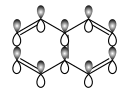
\includegraphics[scale=0.72]{./structures/exercise_1/naphthalene/10.png}
			\captionof*{figure}{$\varepsilon = \alpha + 2.303\beta$}
			\end{minipage} & 
			\begin{minipage}[t]{0.175\linewidth}
			\setlength{\abovecaptionskip}{0.5em}
			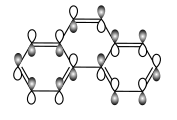
\includegraphics[scale=0.72]{./structures/exercise_1/naphthalene/2.png}
			\captionof*{figure}{$\varepsilon = \alpha + 1.618\beta$}
			\end{minipage} &
			\begin{minipage}[t]{0.175\linewidth}
			\centering
			\setlength{\abovecaptionskip}{0.5em}\hspace*{-0.6em}
			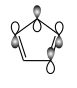
\includegraphics[scale=0.72]{./structures/exercise_1/naphthalene/5.png}
			\captionof*{figure}{$\varepsilon = \alpha + 1.303\beta$}
			\end{minipage} & 
			\begin{minipage}[t]{0.175\linewidth}
			\setlength{\abovecaptionskip}{0.5em}
			\vspace*{-4.8em}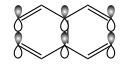
\includegraphics[scale=0.72]{./structures/exercise_1/naphthalene/8.png}\vspace*{0.85em}
			\captionof*{figure}{$\varepsilon = \alpha + 1.000\beta$}
			\end{minipage}
			\begin{minipage}[t]{0.175\linewidth}
			\setlength{\abovecaptionskip}{0.5em}
			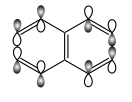
\includegraphics[scale=0.72]{./structures/exercise_1/naphthalene/7.png}\hspace*{-1.5em}
			\captionof*{figure}{$\varepsilon = \alpha + 0.618\beta$}
			\end{minipage} \\
			\begin{minipage}[t]{0.175\linewidth}
			\centering
			\setlength{\abovecaptionskip}{0.5em}
			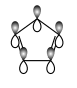
\includegraphics[scale=0.72]{./structures/exercise_1/naphthalene/1.png}
			\captionof*{figure}{$\varepsilon = \alpha -0.618 \beta$}
			\end{minipage} & 
			\begin{minipage}[t]{0.175\linewidth}
			\setlength{\abovecaptionskip}{0.5em}
			\vspace*{-4.7em}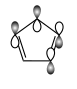
\includegraphics[scale=0.72]{./structures/exercise_1/naphthalene/3.png}\vspace*{0.7em}
			\captionof*{figure}{$\varepsilon = \alpha - 1.000\beta$}
			\end{minipage} &
			\begin{minipage}[t]{0.175\linewidth}
			\centering
			\setlength{\abovecaptionskip}{0.5em}
			\vspace*{-5.5em}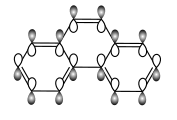
\includegraphics[scale=0.72]{./structures/exercise_1/naphthalene/9.png}
			\captionof*{figure}{$\varepsilon = \alpha - 1.303\beta$}
			\end{minipage} & 
			\begin{minipage}[t]{0.175\linewidth}
			\setlength{\abovecaptionskip}{0.5em}
			\includegraphics[scale=0.72]{./structures/exercise_1/naphthalene/6.png}\hspace*{-0.5em}
			\captionof*{figure}{$\varepsilon = \alpha - 1.618\beta$}
			\end{minipage}
			\begin{minipage}[t]{0.175\linewidth}
			\setlength{\abovecaptionskip}{0.5em}
			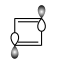
\includegraphics[scale=0.72]{./structures/exercise_1/naphthalene/4.png}\hspace*{-1.5em}
			\captionof*{figure}{$\varepsilon = \alpha - 2.303\beta$}
			\end{minipage}
		\end{tabular}				
		\captionof{figure}{Phase diagrams of these H{\"u}ckel MOs of naphthalene. Black bubbles mean plus phase while white ones mean minus phase. The color is used just for determining relative phase.}\label{fig:phase_diagram_5}
		\end{center}
		
		In the end, we conclude that for naphthalene, its ground state $\pi$-electron configuration is $(1b_{1u})^2 (1b_{2g})^2 (1b_{3g})^2 (2b_{1u})^2 (1a_u)^2$ and its delocalization energy is $2 \times 2.303 \beta + 2 \times 1.618 \beta + 2 \times 1.313 \beta + 2 \times 1.000 \beta + 2 \times 0.618 \beta - 10 \times 1.000 \beta = 3.684 \beta$, much larger than the sum of that of {\it trans}-1,3-butadiene ($0.472\beta$) and benzene ($2.000\beta$). 
		
		\begin{center}
		\includegraphics[scale=1.0]{./structures/exercise_1/naphthalene/998.png}
		\end{center}